\documentclass[12pt]{article}
\usepackage[margin=1in]{geometry}                % See geometry.pdf to learn the layout options. There are lots.
\geometry{letterpaper}                   % ... or a4paper or a5paper or ... 
%\geometry{landscape}                % Activate for for rotated page geometry
\usepackage[parfill]{parskip}    % Activate to begin paragraphs with an empty line rather than an indent

%%%%%%%%%%%%%%%%%%%%
\newcommand{\hide}[1]{}



\usepackage{natbib}
\usepackage{xcolor}
\usepackage{url}
\usepackage{hyperref}
\usepackage{mathtools}
\usepackage[utf8]{inputenc}
\usepackage{float}


\hide{
\usepackage{amscd}
\usepackage{amsfonts}
\usepackage{amsmath}
\usepackage{amssymb}
\usepackage{amsthm}
\usepackage{cases}		 
\usepackage{cutwin}
\usepackage{enumerate}
\usepackage{enumitem}
\usepackage{epstopdf}
\usepackage{graphicx}
\usepackage{ifthen}
\usepackage{lipsum}
\usepackage{mathrsfs}	
\usepackage{multimedia}
\usepackage{wrapfig}
}
\bibliographystyle{humanbio}


\usepackage[utf8]{inputenc}

\newcommand{\itemlist}[1]{\begin{itemize}#1\end{itemize}}
\newcommand{\enumlist}[1]{\begin{enumerate}#1\end{enumerate}}
\newcommand{\desclist}[1]{\begin{description}#1\end{description}}
\newcommand\tab[1][0.5cm]{\hspace*{#1}}

\newcommand{\Answer}[1]{\begin{quote}{\color{blue}#1}\end{quote}}
\newcommand{\AND}{\wedge}
\newcommand{\OR}{\vee}
\newcommand{\ra}{\rightarrow}
\newcommand{\lra}{\leftrightarrow}

\title {{\bf ECE 471 Lab 1} \\
\large{Secret-Key Encryption Lab}}

\author{Mitchell Dzurick}
\date{2/3/2020}
\begin{document}

\maketitle
\textbf{Github with all documentation - \url{https://www.github.com/mitchdz/ECE471}}
\tableofcontents 

\clearpage


Secret Key Encryption Lab

Copyright © 2018 Wenliang Du, Syracuse University. The development of this document was partially funded by the National Science Foundation under Award No. 1303306 and 1718086. This work is licensed under a Creative Commons Attribution-NonCommercial- ShareAlike 4.0 International License. A human-readable summary of (and not a substitute for) the license is the following: You are free to copy and redistribute the material in any medium or format. You must give appropriate credit. If you remix, transform, or build upon the material, you must distribute your contributions under the same license as the original. You may not use the material for commercial purposes.

\section{Overview}

The learning objective of this lab is for students to get familiar with the concepts in the secret-key encryption. After finishing the lab, students should be able to gain a first-hand experience on encryption algorithms, encryption modes, paddings, and initial vector (IV). Moreover, students will be able to use tools and write programs to encrypt/decrypt messages. This lab covers the following topics:

    \begin{itemize}
        \item Secret-key encryption
        \item Substitution cipher and frequency analysis
        \item Encryption modes and paddings
        \item Programming using the crypto library
    \end{itemize}

\textbf{Lab Environment}. This lab has been tested on our pre-built Ubuntu 12.04 VM and Ubuntu 16.04 VM, both of which can be downloaded from the SEED website.

\clearpage

\section{Lab Tasks}
\subsection{Task 1: Frequency c Against Monoalphabetic Substitution Cipher}
    
It is well-known that monoalphabetic substitution cipher (also known as monoalphabetic cipher) is not secure, because it can be subjected to frequency analysis. In this lab, you are given a cipher-text that is encrypted using a monoalphabetic cipher; namely, each letter in the original text is replaced by another letter, where the replacement does not vary (i.e., a letter is always replaced by the same letter during the encryption). Your job is to find out the original text using frequency analysis. It is known that the original text is an English article.

\subsubsection{Task 1: solution}

Shown below is the linux command 
\begin{verbatim}
    $ ls -l 
\end{verbatim}
in the lab1/task1 directory of my github repository. Inside that repository, the following command is used to copy the contents of the ciphertext into my X clipboard:
\begin{verbatim}
    $ xclip -sel clip -i ciphertext.txt
\end{verbatim}

% Figure~\ref{fig:foo}
\begin{figure}[!ht]
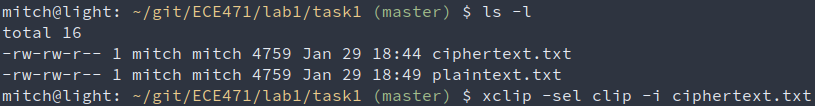
\includegraphics[scale=0.65]{c0.png}
\caption{listing of lab1/task1 directory}
\label{fig:c0}
\end{figure}


The contents of ciphertext.txt is copied below:
\begin{verbatim}
ytn xqavhq yzhu  xu qzupvd ltmat qnncq vgxzy hmrty vbynh ytmq ixur qyhvurn
vlvhpq yhme ytn gvrrnh bnniq imsn v uxuvrnuvhmvu yxx

ytn vlvhpq hvan lvq gxxsnupnp gd ytn pncmqn xb tvhfnd lnmuqynmu vy myq xzyqny
vup ytn veevhnuy mceixqmxu xb tmq bmic axcevud vy ytn nup vup my lvq qtvenp gd
ytn ncnhrnuan xb cnyxx ymcnq ze givasrxlu eximymaq vhcavupd vaymfmqc vup
v uvymxuvi axufnhqvymxu vq ghmnb vup cvp vq v bnfnh phnvc vgxzy ltnytnh ytnhn
xzrty yx gn v ehnqmpnuy lmubhnd ytn qnvqxu pmpuy ozqy qnnc nkyhv ixur my lvq
nkyhv ixur gnavzqn ytn xqavhq lnhn cxfnp yx ytn bmhqy lnnsnup mu cvhat yx
vfxmp axubimaymur lmyt ytn aixqmur anhncxud xb ytn lmuynh xidcemaq ytvusq
ednxuratvur

xun gmr jznqymxu qzhhxzupmur ytmq dnvhq vavpncd vlvhpq mq txl xh mb ytn
anhncxud lmii vpphnqq cnyxx nqenamviid vbynh ytn rxipnu rixgnq ltmat gnavcn
v ozgmivuy axcmurxzy evhyd bxh ymcnq ze ytn cxfncnuy qenvhtnvpnp gd 
exlnhbzi txiidlxxp lxcnu ltx tnienp hvmqn cmiimxuq xb pxiivhq yx bmrty qnkzvi
tvhvqqcnuy vhxzup ytn axzuyhd

qmruvimur ytnmh qzeexhy rxipnu rixgnq vyynupnnq qlvytnp ytncqnifnq mu givas
qexhynp iveni emuq vup qxzupnp xbb vgxzy qnkmqy exlnh mcgvivuanq bhxc ytn hnp
avheny vup ytn qyvrn xu ytn vmh n lvq aviinp xzy vgxzy evd munjzmyd vbynh
myq bxhcnh vuatxh avyy qvpinh jzmy xuan qtn invhunp ytvy qtn lvq cvsmur bvh
inqq ytvu v cvin axtxqy vup pzhmur ytn anhncxud uvyvimn exhycvu yxxs v gizuy
vup qvymqbdmur pmr vy ytn viicvin hxqynh xb uxcmuvynp pmhnayxhq txl axzip
ytvy gn yxeenp

vq my yzhuq xzy vy invqy mu ynhcq xb ytn xqavhq my ehxgvgid lxuy gn

lxcnu mufxifnp mu ymcnq ze qvmp ytvy viytxzrt ytn rixgnq qmrumbmnp ytn
mumymvymfnq ivzuat ytnd unfnh muynupnp my yx gn ozqy vu vlvhpq qnvqxu
avcevmru xh xun ytvy gnavcn vqqxamvynp xuid lmyt hnpavheny vaymxuq muqynvp
v qexsnqlxcvu qvmp ytn rhxze mq lxhsmur gntmup aixqnp pxxhq vup tvq qmuan
vcvqqnp  cmiimxu bxh myq inrvi pnbnuqn bzup ltmat vbynh ytn rixgnq lvq
bixxpnp lmyt ytxzqvupq xb pxuvymxuq xb  xh inqq bhxc enxein mu qxcn 
axzuyhmnq


ux avii yx lnvh givas rxluq lnuy xzy mu vpfvuan xb ytn xqavhq ytxzrt ytn
cxfncnuy lmii vicxqy anhyvmuid gn hnbnhnuanp gnbxhn vup pzhmur ytn anhncxud 
nqenamviid qmuan fxavi cnyxx qzeexhynhq imsn vqtind ozpp ivzhv pnhu vup
umaxin smpcvu vhn qatnpzinp ehnqnuynhq

vuxytnh bnvyzhn xb ytmq qnvqxu ux xun hnviid suxlq ltx mq rxmur yx lmu gnqy
emayzhn vhrzvgid ytmq tveenuq v ixy xb ytn ymcn muvhrzvgid ytn uvmigmynh
uvhhvymfn xuid qnhfnq ytn vlvhpq tden cvatmun gzy xbynu ytn enxein bxhnavqymur
ytn hvan qxaviinp xqavhxixrmqyq avu cvsn xuid npzavynp rznqqnq

ytn lvd ytn vavpncd yvgzivynq ytn gmr lmuunh pxnquy tnie mu nfnhd xytnh
avynrxhd ytn uxcmunn lmyt ytn cxqy fxynq lmuq gzy mu ytn gnqy emayzhn
avynrxhd fxynhq vhn vqsnp yx imqy ytnmh yxe cxfmnq mu ehnbnhnuymvi xhpnh mb v
cxfmn rnyq cxhn ytvu  enhanuy xb ytn bmhqyeivan fxynq my lmuq ltnu ux
cxfmn cvuvrnq ytvy ytn xun lmyt ytn bnlnqy bmhqyeivan fxynq mq nimcmuvynp vup
myq fxynq vhn hnpmqyhmgzynp yx ytn cxfmnq ytvy rvhunhnp ytn nimcmuvynp gviixyq
qnaxupeivan fxynq vup ytmq axuymuznq zuymi v lmuunh ncnhrnq

my mq vii ynhhmgid axubzqmur gzy veevhnuyid ytn axuqnuqzq bvfxhmyn axcnq xzy
vtnvp mu ytn nup ytmq cnvuq ytvy nupxbqnvqxu vlvhpq atvyynh mufvhmvgid
mufxifnq yxhyzhnp qenazivymxu vgxzy ltmat bmic lxzip cxqy imsnid gn fxynhq
qnaxup xh ytmhp bvfxhmyn vup ytnu njzviid yxhyzhnp axuaizqmxuq vgxzy ltmat
bmic cmrty ehnfvmi

mu  my lvq v yxqqze gnylnnu gxdtxxp vup ytn nfnuyzvi lmuunh gmhpcvu
mu  lmyt ixyq xb nkenhyq gnyymur xu ytn hnfnuvuy xh ytn gmr qtxhy ytn
ehmwn lnuy yx qexyimrty ivqy dnvh unvhid vii ytn bxhnavqynhq pnaivhnp iv
iv ivup ytn ehnqzceymfn lmuunh vup bxh ylx vup v tvib cmuzynq ytnd lnhn
axhhnay gnbxhn vu nufnixen quvbz lvq hnfnvinp vup ytn hmrtybzi lmuunh
cxxuimrty lvq ahxlunp

ytmq dnvh vlvhpq lvyatnhq vhn zunjzviid pmfmpnp gnylnnu ythnn gmiigxvhpq
xzyqmpn nggmur cmqqxzhm ytn bvfxhmyn vup ytn qtven xb lvynh ltmat mq
ytn gvrrnhq ehnpmaymxu lmyt v bnl bxhnavqymur v tvmi cvhd lmu bxh rny xzy

gzy vii xb ytxqn bmicq tvfn tmqyxhmavi xqavhfxymur evyynhuq vrvmuqy ytnc ytn
qtven xb lvynh tvq  uxcmuvymxuq cxhn ytvu vud xytnh bmic vup lvq viqx
uvcnp ytn dnvhq gnqy gd ytn ehxpzanhq vup pmhnayxhq rzmipq dny my lvq uxy
uxcmuvynp bxh v qahnnu vayxhq rzmip vlvhp bxh gnqy nuqncgin vup ux bmic tvq
lxu gnqy emayzhn lmytxzy ehnfmxzqid ivupmur vy invqy ytn vayxhq uxcmuvymxu
qmuan ghvfntnvhy mu  ytmq dnvh ytn gnqy nuqncgin qvr nupnp ze rxmur yx
ythnn gmiigxvhpq ltmat mq qmrumbmavuy gnavzqn vayxhq cvsn ze ytn vavpncdq
ivhrnqy ghvuat ytvy bmic ltmin pmfmqmfn viqx lxu ytn gnqy phvcv rxipnu rixgn
vup ytn gvbyv gzy myq bmiccvsnh cvhymu capxuvrt lvq uxy uxcmuvynp bxh gnqy
pmhnayxh vup vevhy bhxc vhrx cxfmnq ytvy ivup gnqy emayzhn lmytxzy viqx
nvhumur gnqy pmhnayxh uxcmuvymxuq vhn bnl vup bvh gnylnnu
\end{verbatim}

The related plaintext is shown below using the final (substitution) key `abcdefghijklmnopqrstuvwxyz` to `cfmypvbrlqxwiejdsgkhnazotu`. The process to derive this key is outlined below with accompanying pictures.

\begin{figure}[H]
    \begin{center}
        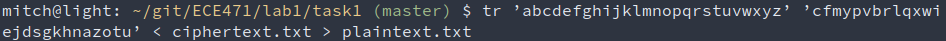
\includegraphics[scale=0.5]{c23.png}
    \end{center}{}
    \caption{Command to convert ciphertext to plaintext}
    \label{fig:c23}
\end{figure}

Figure~\ref{fig:c23} shows the linux command used to convert the ciphertex that was shown into the accompanying plaintext.

\begin{verbatim}
the oscars turn  on sunday which seems about right after this long strange
awards trip the bagger feels like a nonagenarian too

the awards race was bookended by the demise of harvey weinstein at its outset
and the apparent implosion of his film company at the end and it was shaped by
the emergence of metoo times up blackgown politics armcandy activism and
a national conversation as brief and mad as a fever dream about whether there
ought to be a president winfrey the season didnt just seem extra long it was
extra long because the oscars were moved to the first weekend in march to
avoid conflicting with the closing ceremony of the winter olympics thanks
pyeongchang

one big question surrounding this years academy awards is how or if the
ceremony will address metoo especially after the golden globes which became
a jubilant comingout party for times up the movement spearheaded by 
powerful hollywood women who helped raise millions of dollars to fight sexual
harassment around the country

signaling their support golden globes attendees swathed themselves in black
sported lapel pins and sounded off about sexist power imbalances from the red
carpet and the stage on the air e was called out about pay inequity after
its former anchor catt sadler quit once she learned that she was making far
less than a male cohost and during the ceremony natalie portman took a blunt
and satisfying dig at the allmale roster of nominated directors how could
that be topped

as it turns out at least in terms of the oscars it probably wont be

women involved in times up said that although the globes signified the
initiatives launch they never intended it to be just an awards season
campaign or one that became associated only with redcarpet actions instead
a spokeswoman said the group is working behind closed doors and has since
amassed  million for its legal defense fund which after the globes was
flooded with thousands of donations of  or less from people in some 
countries


no call to wear black gowns went out in advance of the oscars though the
movement will almost certainly be referenced before and during the ceremony 
especially since vocal metoo supporters like ashley judd laura dern and
nicole kidman are scheduled presenters

another feature of this season no one really knows who is going to win best
picture arguably this happens a lot of the time inarguably the nailbiter
narrative only serves the awards hype machine but often the people forecasting
the race socalled oscarologists can make only educated guesses

the way the academy tabulates the big winner doesnt help in every other
category the nominee with the most votes wins but in the best picture
category voters are asked to list their top movies in preferential order if a
movie gets more than  percent of the firstplace votes it wins when no
movie manages that the one with the fewest firstplace votes is eliminated and
its votes are redistributed to the movies that garnered the eliminated ballots
secondplace votes and this continues until a winner emerges

it is all terribly confusing but apparently the consensus favorite comes out
ahead in the end this means that endofseason awards chatter invariably
involves tortured speculation about which film would most likely be voters
second or third favorite and then equally tortured conclusions about which
film might prevail

in  it was a tossup between boyhood and the eventual winner birdman
in  with lots of experts betting on the revenant or the big short the
prize went to spotlight last year nearly all the forecasters declared la
la land the presumptive winner and for two and a half minutes they were
correct before an envelope snafu was revealed and the rightful winner
moonlight was crowned

this year awards watchers are unequally divided between three billboards
outside ebbing missouri the favorite and the shape of water which is
the baggers prediction with a few forecasting a hail mary win for get out

but all of those films have historical oscarvoting patterns against them the
shape of water has  nominations more than any other film and was also
named the years best by the producers and directors guilds yet it was not
nominated for a screen actors guild award for best ensemble and no film has
won best picture without previously landing at least the actors nomination
since braveheart in  this year the best ensemble sag ended up going to
three billboards which is significant because actors make up the academys
largest branch that film while divisive also won the best drama golden globe
and the bafta but its filmmaker martin mcdonagh was not nominated for best
director and apart from argo movies that land best picture without also
earning best director nominations are few and far between
\end{verbatim}

After the ciphertext is copied, a program is utilized that is supplied by cryptoclub.org. The domain is shown below.

\begin{figure}[!ht]
    \begin{center}
        
\includegraphics[scale=0.65]{c0.1.png}
    \end{center}{}
    \caption{cryptoclub website}
    \label{fig:c0.1}
\end{figure}

\clearpage

Below is the page you should see upon opening the URL in Figure~\ref{fig:c0.1}

\begin{figure}[!ht]
    \begin{center}
        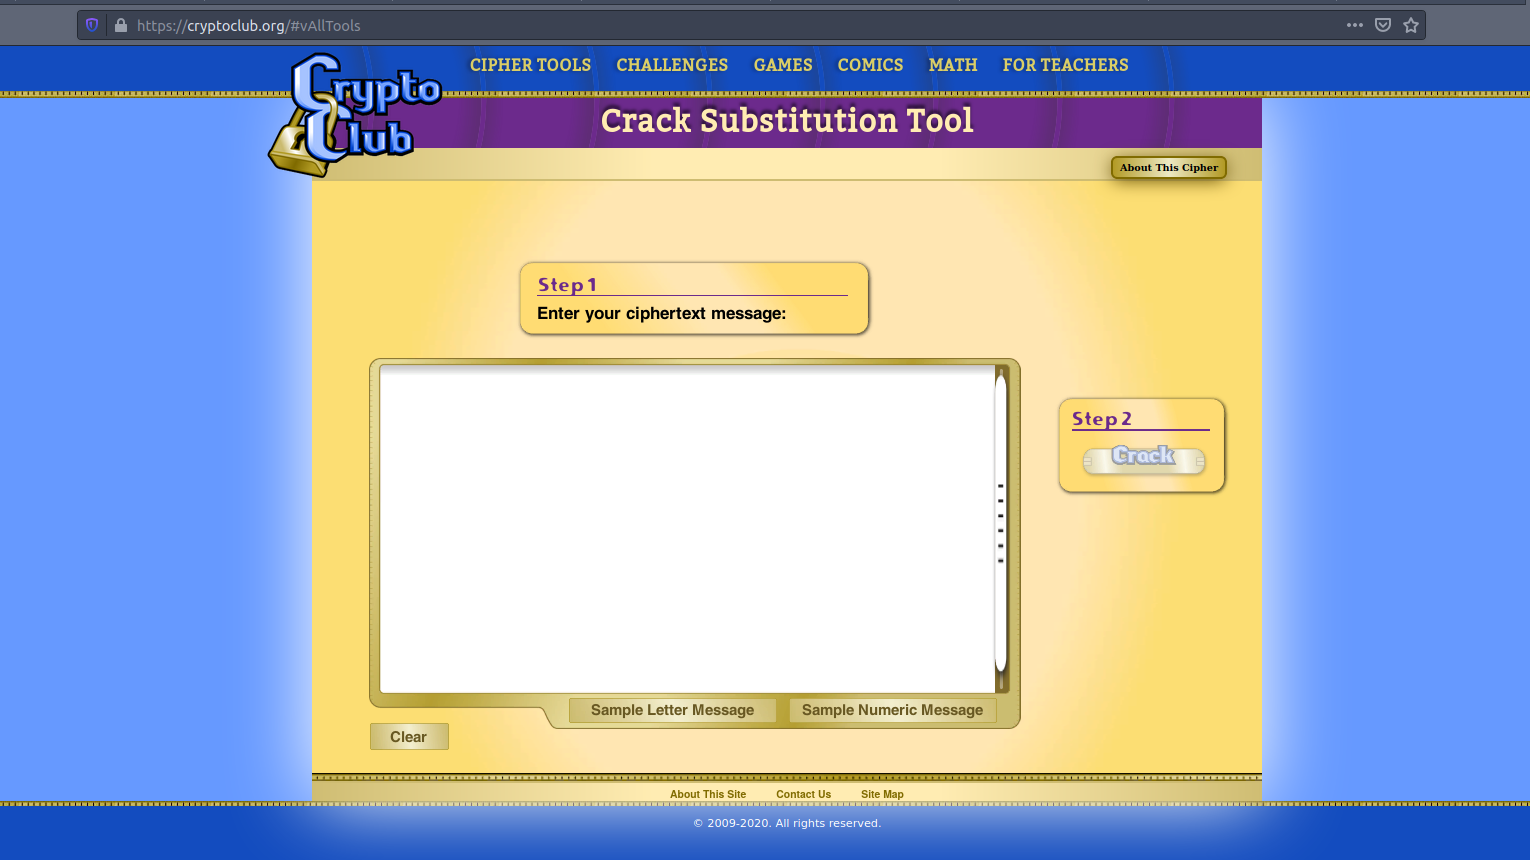
\includegraphics[scale=0.3]{c1.png}
    \end{center}{}
    \caption{cryptoclub main page}
    \label{fig:c1}
\end{figure}


The contents of the ciphertext are copied into the program as shown in Figure~\ref{fig:c3}. On this page, the ciphertext shows the frequency of letters and relates the frequency of letters in the ciphertext to the frequency of letters in the English alphabet.


\begin{figure}[!ht]
    \begin{center}
        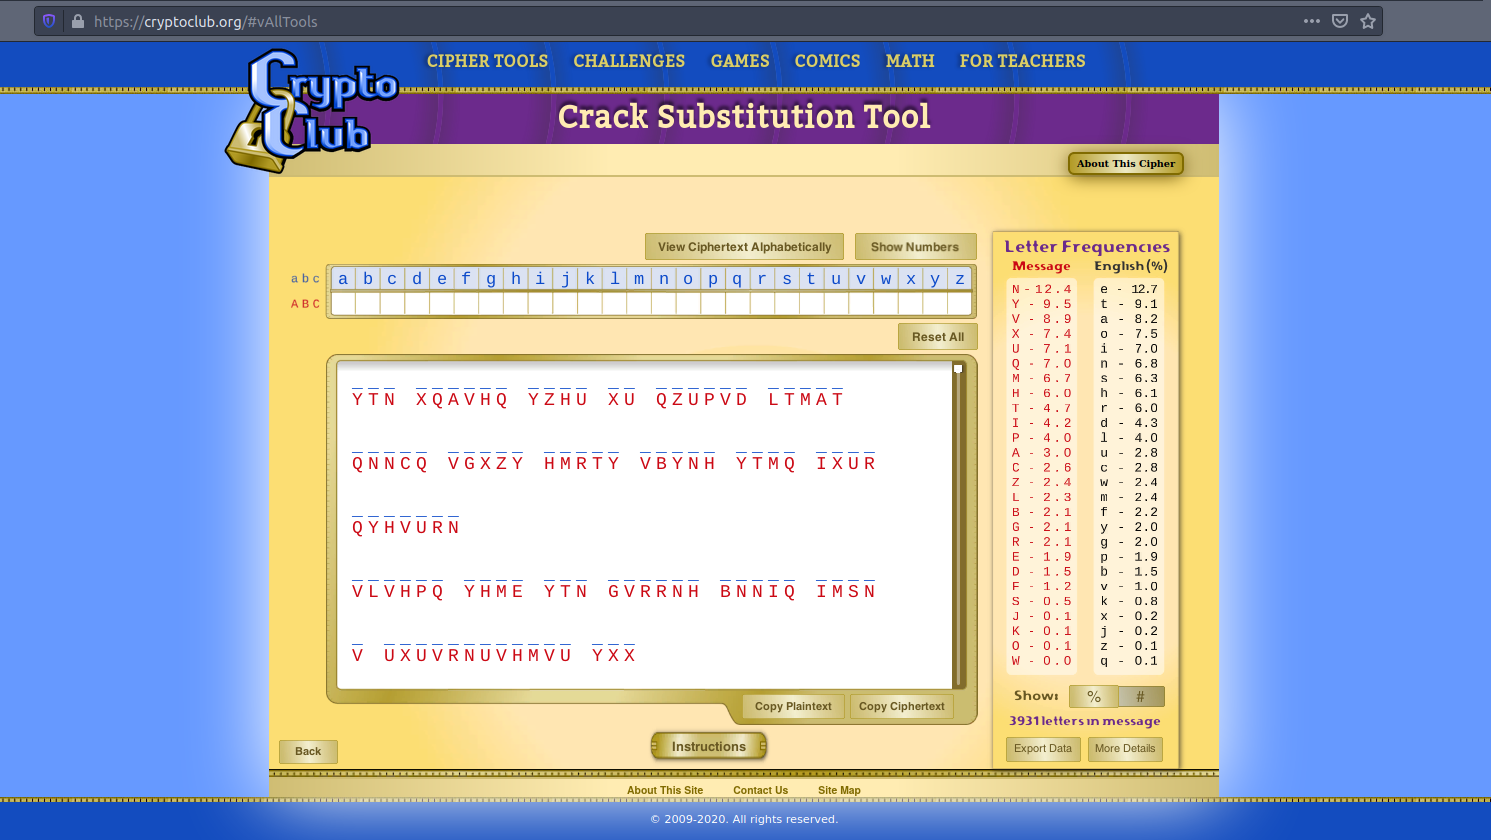
\includegraphics[scale=0.3]{c3.png}
    \end{center}{}
    \caption{Crack Substitution Tool main page}
    \label{fig:c3}
\end{figure}

\begin{figure}[H]
    \begin{center}
        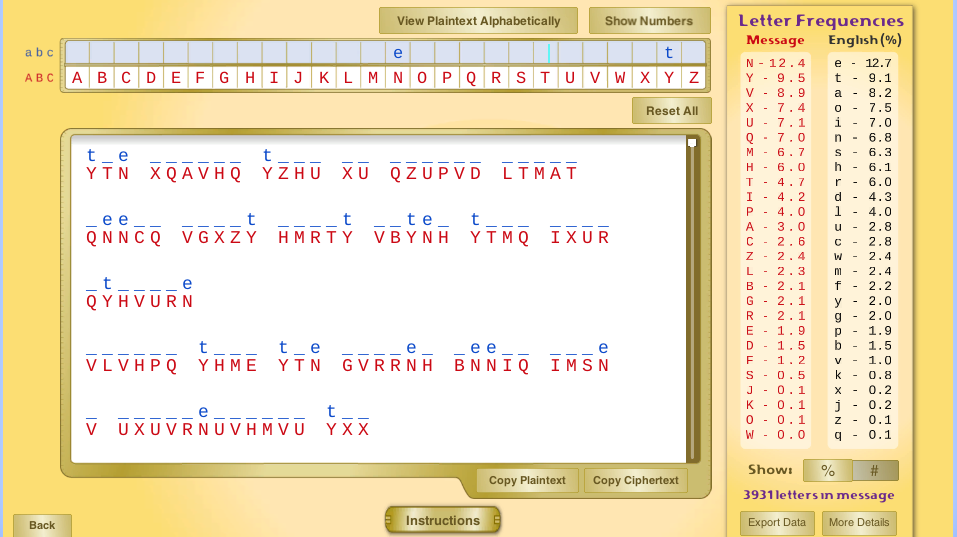
\includegraphics[scale=0.48]{c4.png}
    \end{center}{}
    \caption{Mapping N to e and Y to t}
    \label{fig:c4}
\end{figure}

In Figure~\ref{fig:c4} N is mapped to `e` and Y is mapped to `t` due to frequency analysis (You can see that N matches e and Y matches t in frequency on the right). It is very easy then to notice that T maps to `h` shown in Figure~\ref{fig:c5} to create the Trigram `the`.

\begin{figure}[H]
    \begin{center}
        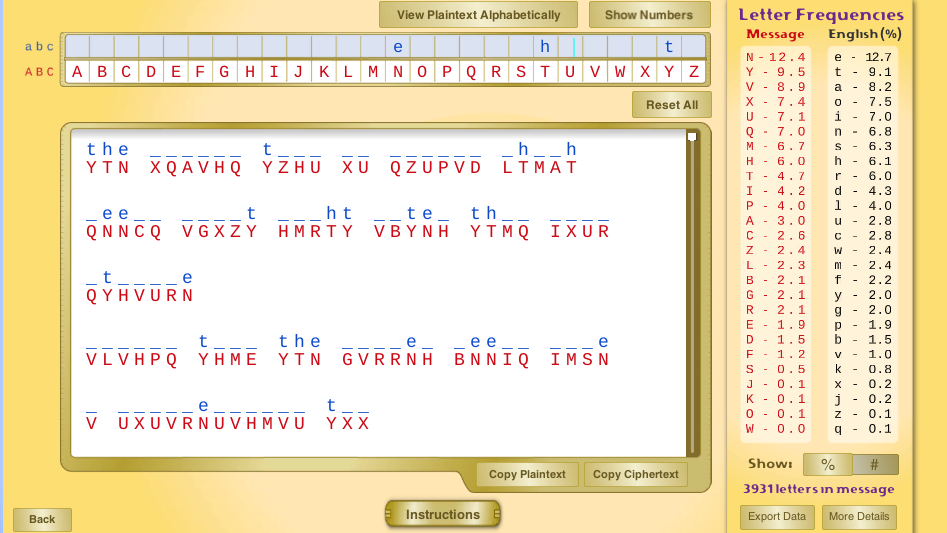
\includegraphics[scale=0.48]{c5.png}
    \end{center}{}
    \caption{Mapping T to h}
    \label{fig:c5}
\end{figure}


\begin{figure}[H]
    \begin{center}
        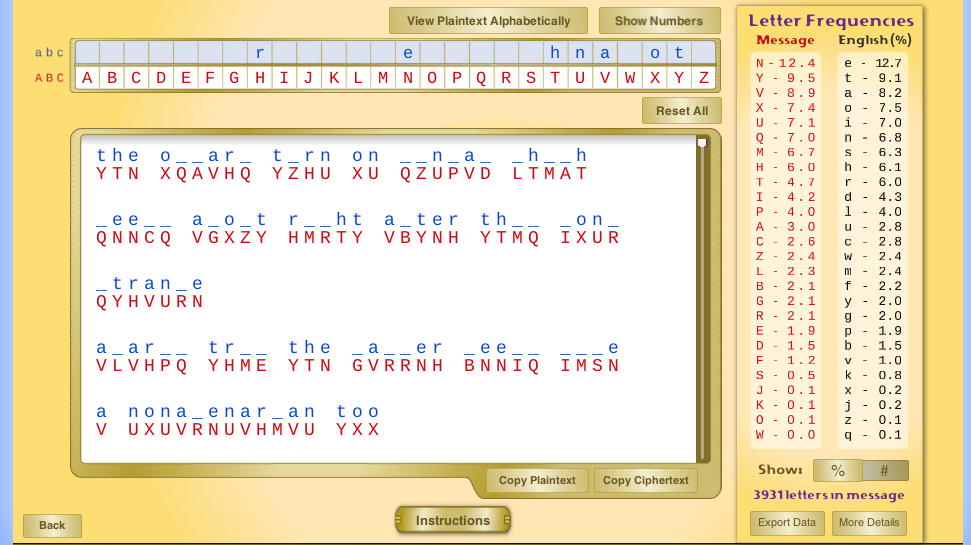
\includegraphics[scale=0.48]{c6.png}
    \end{center}{}
    \caption{Mapping U to n, V to a, X to o, and H to r}
    \label{fig:c6}
\end{figure}

Figure~\ref{fig:c6} shows how the ciphertext letters `UVXH` are mapped to `naor`. This mapping was done by looking at the ciphertext frequency and mapping the frequency to the closest related frequency in the english alphabet. Words do not particularly make sense yet, so it is just assumed for now that this is the correct mapping.



\begin{figure}[H]
    \begin{center}
        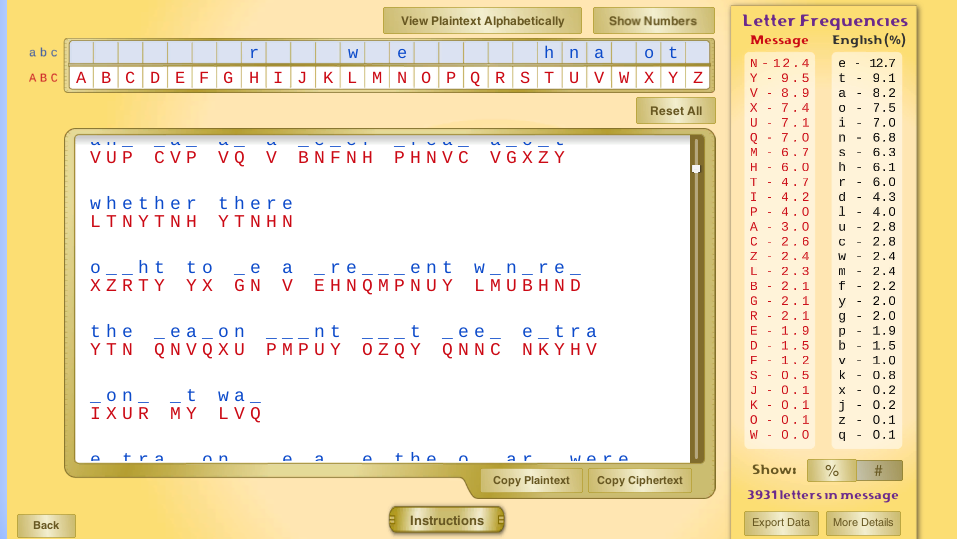
\includegraphics[scale=0.48]{c7.png}
    \end{center}{}
    \caption{mapping L to w}
    \label{fig:c7}
\end{figure}


In Figure~\ref{fig:c7} the string `hether` was shown, which clearly meant to spell `whether`. Therefore, L maps to w.

\begin{figure}[H]
    \begin{center}
        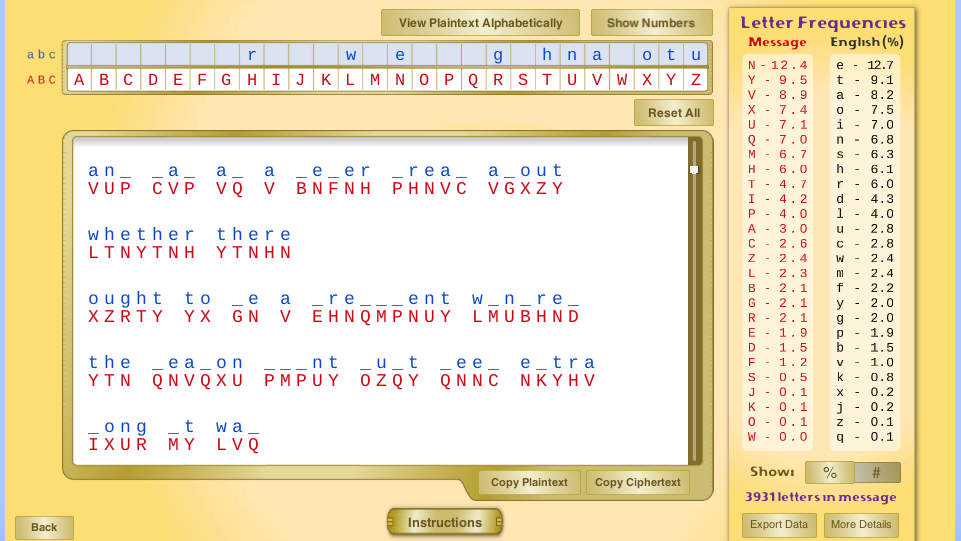
\includegraphics[scale=0.48]{c8.png}
    \end{center}{}
    \caption{Mapping R to g}
    \label{fig:c8}
\end{figure}

In Figure~\ref{fig:c8} the string 'ou-ht' is shown, which is meant to say 'ought'. Therefore, R maps to g.

\begin{figure}[H]
    \begin{center}
        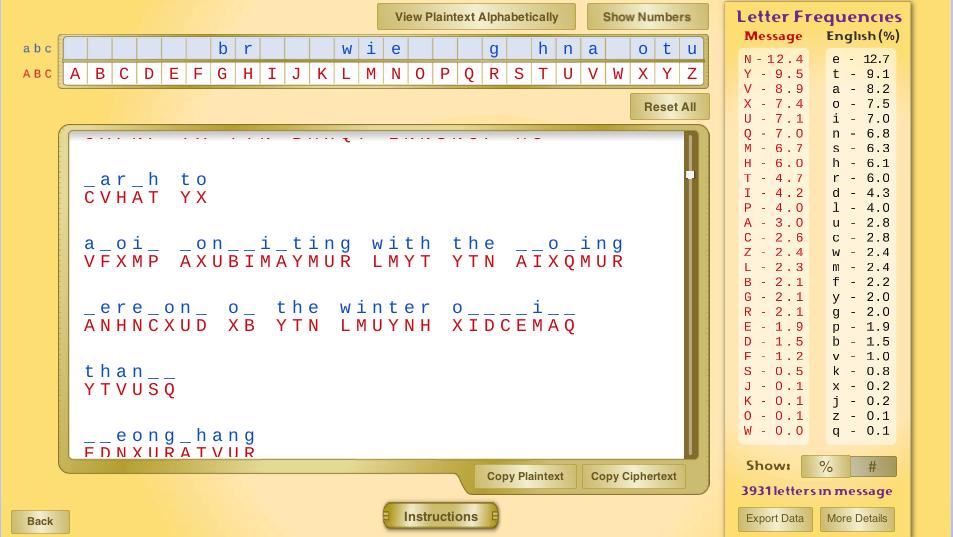
\includegraphics[scale=0.48]{c9.png}
    \end{center}{}
    \caption{Mapping G to b and M to i}
    \label{fig:c9}
\end{figure}

In Figure~\ref{fig:c9} The string 'w-nter' was shown, which should mean 'winter', Thus M maps to i. The mapping for G to b is not shown in this picture, but was done in a very similar fashion with another word.

\begin{figure}[H]
    \begin{center}
        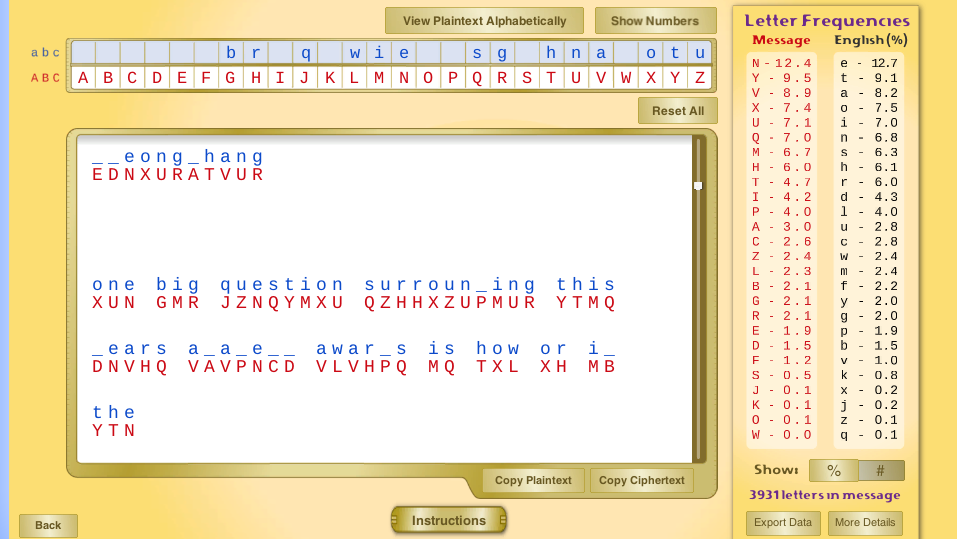
\includegraphics[scale=0.48]{c10.png}
    \end{center}{}
    \caption{Mapping J to q and Q to s}
    \label{fig:c10}
\end{figure}

In Figure~\ref{fig:c10} The string '-ue-tion' was present, which obviously meant 'question', therefore J maps to q & Q maps to s.


\begin{figure}[H]
    \begin{center}
        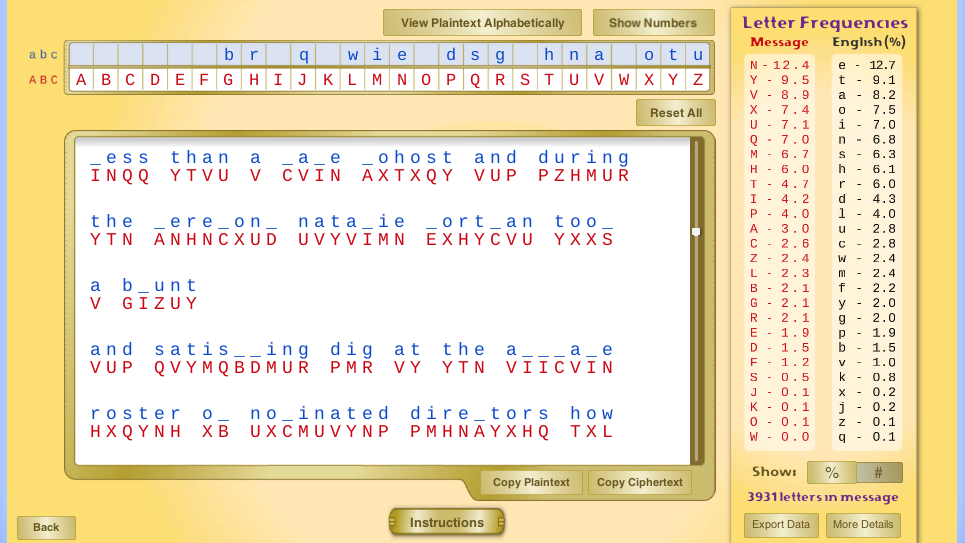
\includegraphics[scale=0.48]{c11.png}
    \end{center}{}
    \caption{Mapping P to d}
    \label{fig:c11}
\end{figure}

In Figure~\ref{fig:c11} The string 'an-' and '-ig' and '-uring' was present. Therefore, it is clear that P maps to d.

\begin{figure}[H]
    \begin{center}
        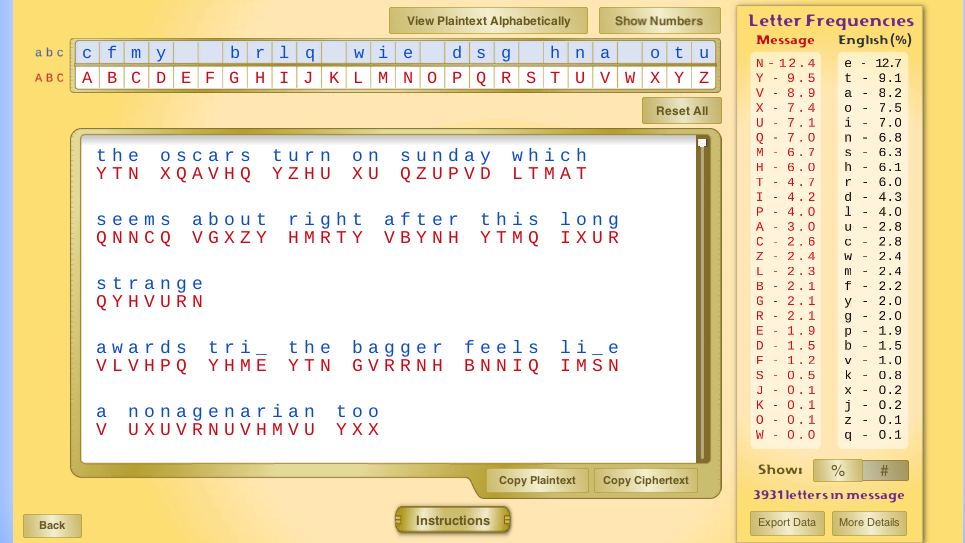
\includegraphics[scale=0.48]{c12.png}
    \end{center}{}
    \caption{Mapping A to c, B to f, C to m, D to y, and I to l}
    \label{fig:c12}
\end{figure}

In Figure~\ref{fig:c12} there are a lot of substitutions made. In particular, substitution A to c, B to f, C to m, D to y, and I to l. 'sunda-' was present which lead D to map to y, 'fee-s' which mapped I to l, 'os-ars' which mapped A to c, and the mapping from C to m is not present in Figure~\ref{fig:c12}, but was done in a much similar fashion.

\begin{figure}[H]
    \begin{center}
        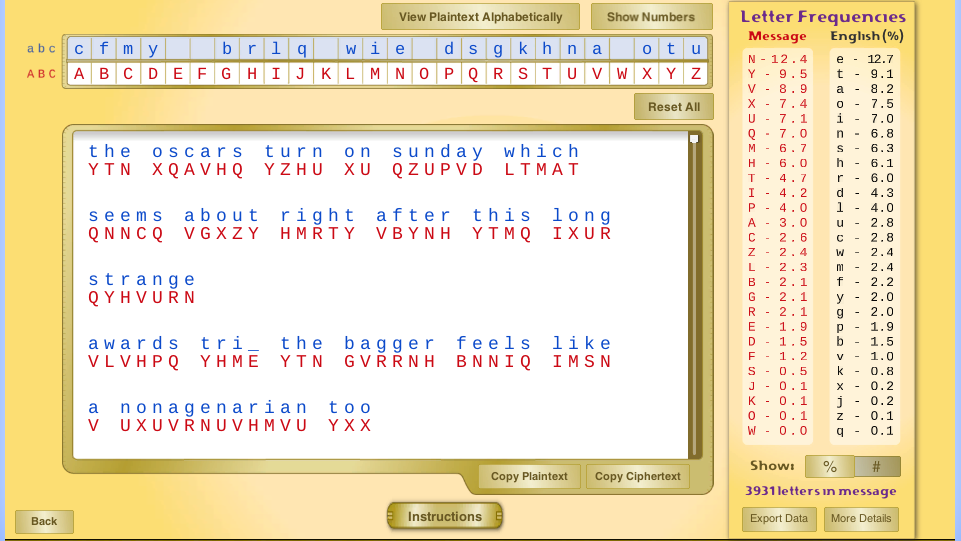
\includegraphics[scale=0.48]{c13.png}
    \end{center}{}
    \caption{Mapping S to k}
    \label{fig:c13}
\end{figure}

In figure~\ref{fig:c13} the mapping from S to k was done. This is due to the work 'li-e' being present, which is \emph{likely} to be 'like'. Therefore, S maps to K. (get the pun)


\begin{figure}[H]
    \begin{center}
        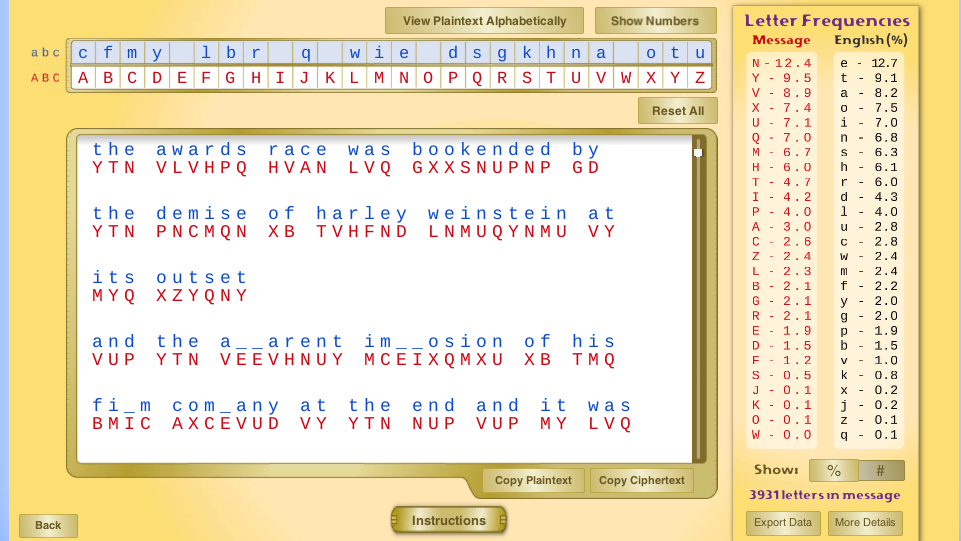
\includegraphics[scale=0.48]{c14.png}
    \end{center}{}
    \caption{mapping F to l, removing I to l}
    \label{fig:c14}
\end{figure}

In Figure~\ref{fig:c14} F is now mapped to l because the assumption was that the string 'harley' needed to be made. This removed the mapping from I to l.

\begin{figure}[H]
    \begin{center}
        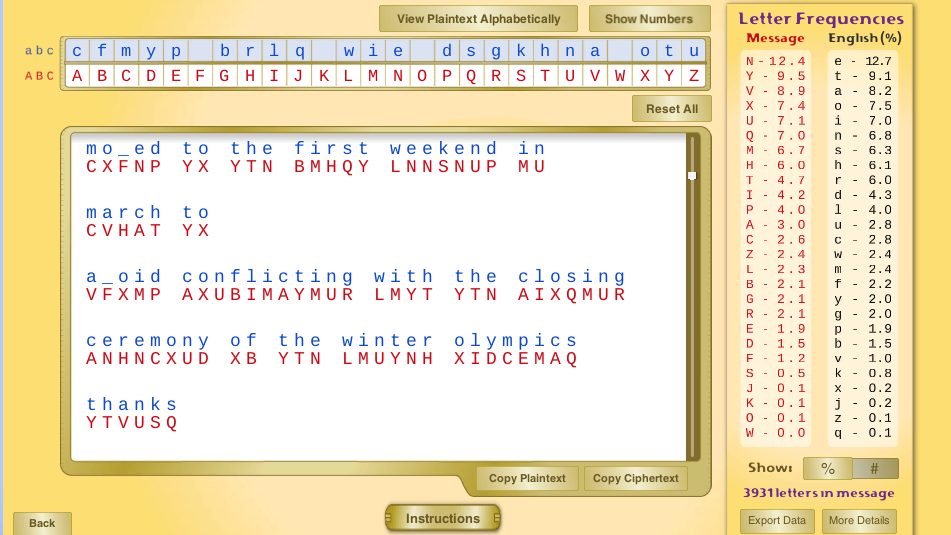
\includegraphics[scale=0.48]{c15.png}
    \end{center}{}
    \caption{Mapping E to p, and re-mapping I to l}
    \label{fig:c15}
\end{figure}

In Figure~\ref{fig:c15} E is mapped to p because 'olym-ics' was present, which definitely meains olympics. It was also noted that I should definitly be L because the string 'with the c-osing ceremony' was present.


\begin{figure}[H]
    \begin{center}
        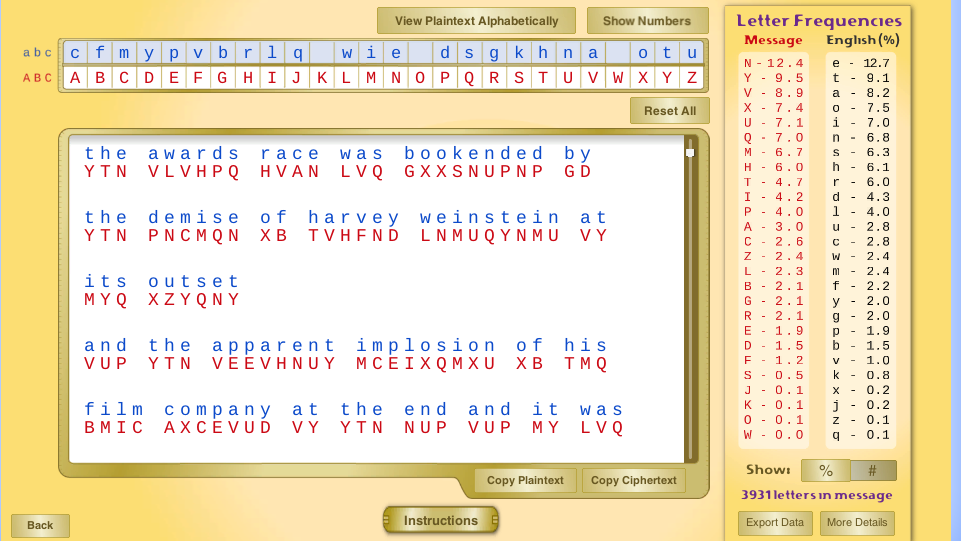
\includegraphics[scale=0.48]{c16.png}
    \end{center}{}
    \caption{Mapping F to v}
    \label{fig:c16}
\end{figure}

In Figure~\ref{fig:c16} it is clear that F should be mapped to v now, and that 'har-ey' should be 'harvey' to complete the name Harvery Weinstein.


\begin{figure}[H]
    \begin{center}
        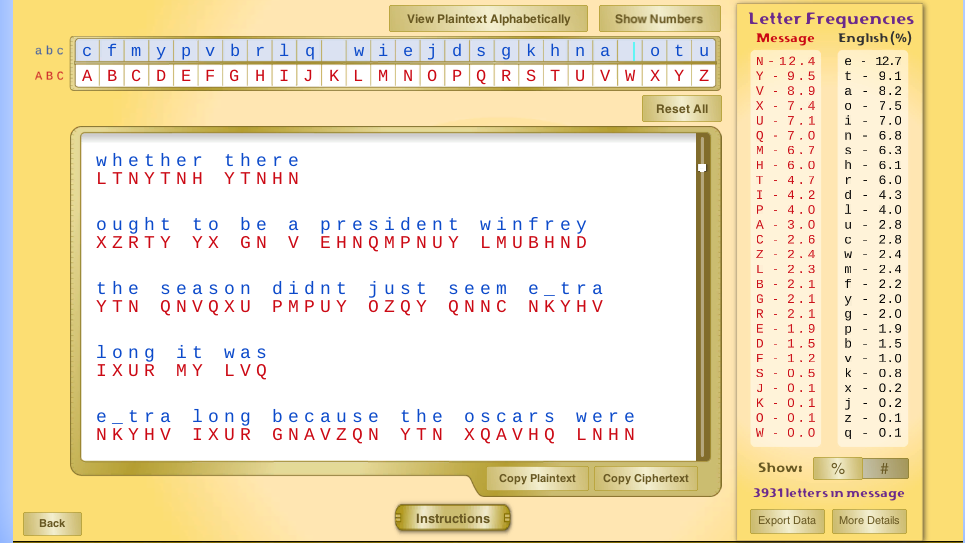
\includegraphics[scale=0.48]{c17.png}
    \end{center}{}
    \caption{Mapping O to j}
    \label{fig:c17}
\end{figure}

In Figure~\ref{fig:c17} it is clear that O should be mapped to j because the phrase 'the season didnt -ust seem' which obviously meant to say just.


\begin{figure}[H]
    \begin{center}
        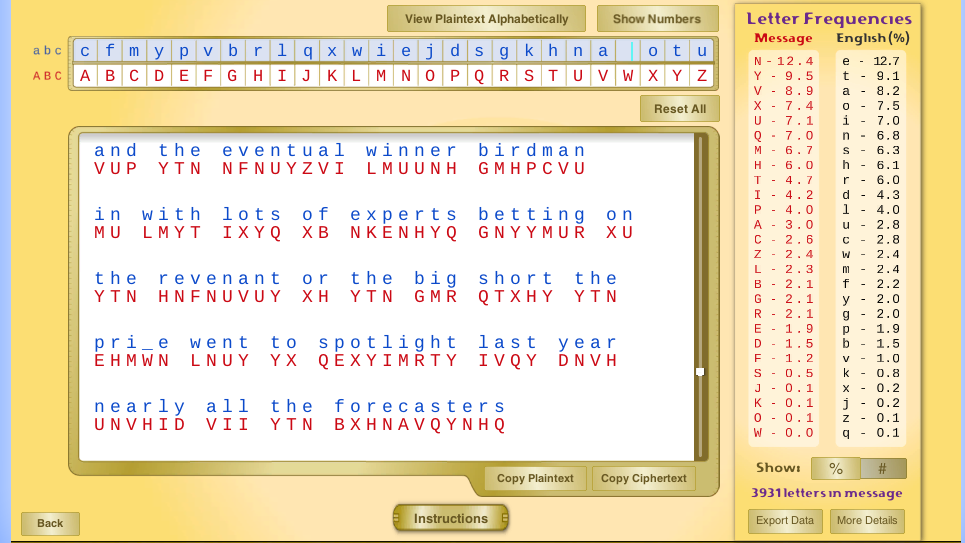
\includegraphics[scale=0.48]{c18.png}
    \end{center}{}
    \caption{Mapping K to x}
    \label{fig:c18}
\end{figure}

In Figure~\ref{fig:c18} it is clear that K should map x because the string 'e-perts' is present which should map to 'experts'.

\begin{figure}[H]
    \begin{center}
        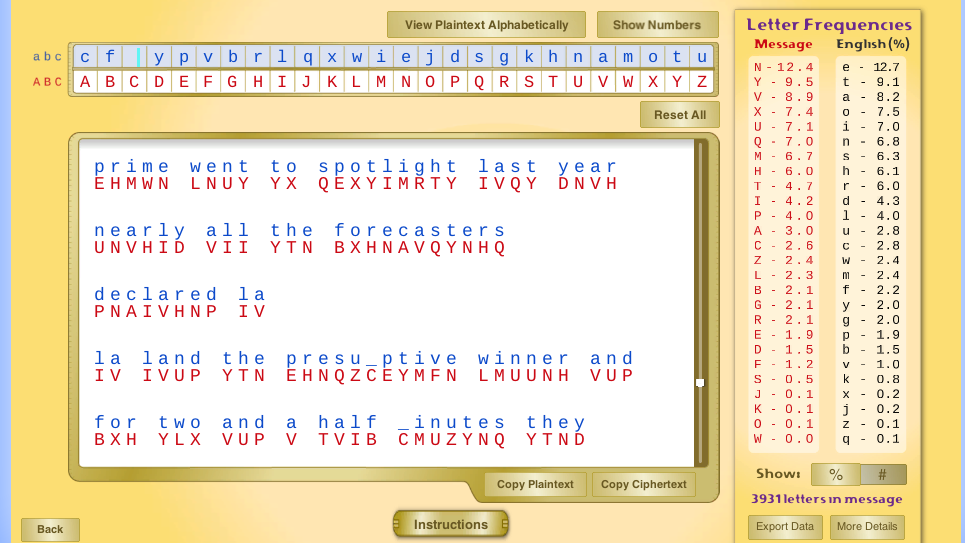
\includegraphics[scale=0.48]{c19.png}
    \end{center}{}
    \caption{Mapping W to m, removing C to m}
    \label{fig:c19}
\end{figure}

In Figure~\ref{fig:c19} it is clear that W should map to `m` because the string 'pri-e' is present which is referring to 'prime'

\begin{figure}[H]
    \begin{center}
        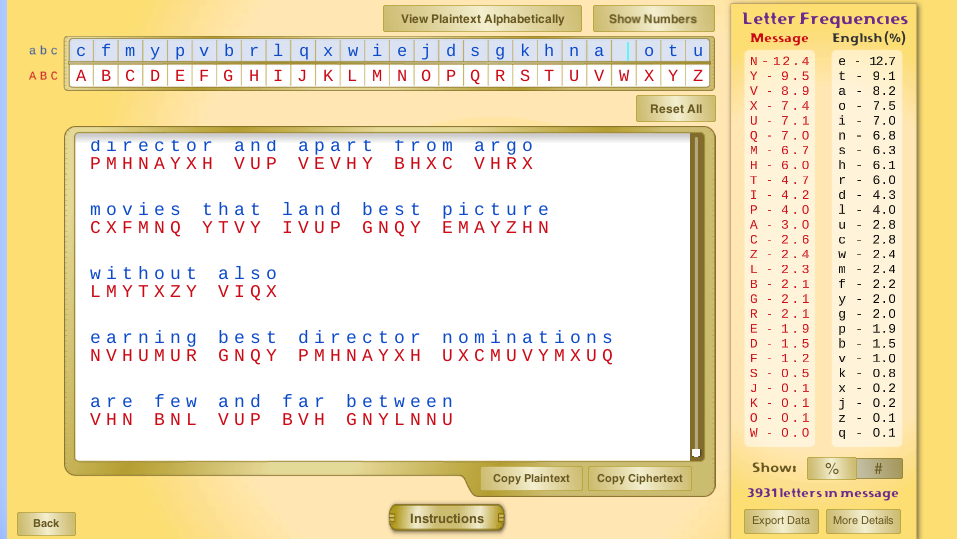
\includegraphics[scale=0.48]{c20.png}
    \end{center}{}
    \caption{mapping C to m and removing W to m}
    \label{fig:c20}
\end{figure}

In Figure~\ref{fig:c20} It is now really clear that mapping W to m was a mistake because the string 'fro- argo -ovies that' which maps to 'from argo movies that'.

\begin{figure}[!ht]
    \begin{center}
        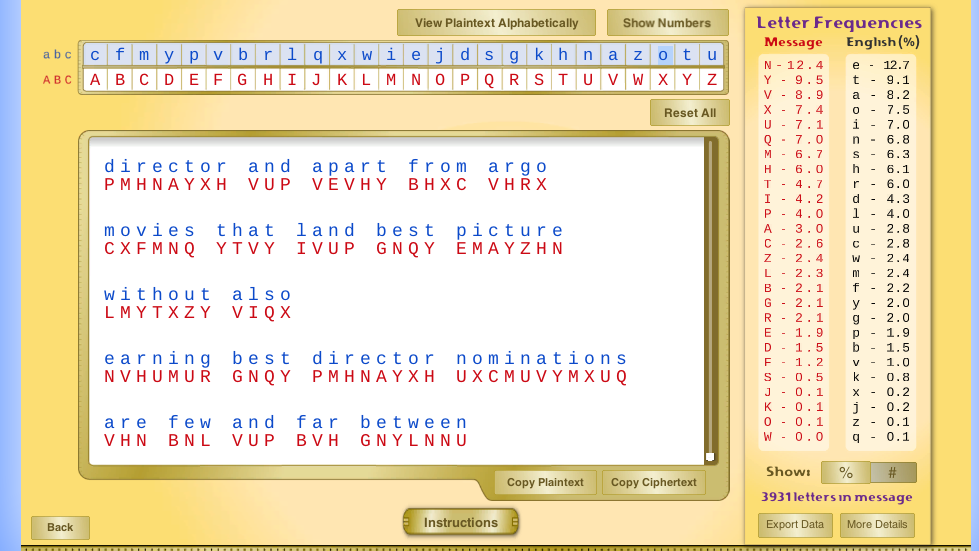
\includegraphics[scale=0.48]{c21.png}
    \end{center}{}
    \caption{Mapping W to z}
    \label{fig:c21}
\end{figure}

In Figure~\ref{fig:c21} W maps to z due to the process of elimination, because W does not show up, and neither does Z.


Finally, the key `abcdefghijklmnopqrstuvwxyz` to `cfmypvbrlqxwiejdsgkhnazotu` is obtained, where the first string `abcdefghijklmnopqrstuvwxyz` is the ciphertext letters.

\subsection{Task 2: Encryption using Different Ciphers and Modes}

In this task, we will play with various encryption algorithms and modes. You can use the following
openssl enc command to encrypt/decrypt a file. To see the manuals, you can type man openssl
and man enc.

\begin{verbatim}
openssl enc -ciphertype -e -in plain.txt -out cipher.bin \
    -K 00112233445566778889aabbccddeeff \
    -iv 0102030405060708SEED 
\end{verbatim}

Please replace the ciphertype with a specific cipher type, such as -aes-128-cbc, -bf-cbc,
-aes-128-cfb, etc. In this task, you should try at least 3 different ciphers. You can find the meaning
of the command-line options and all the supported cipher types by typing "man enc". We include some
common options for the openssl enc command in the following:
\begin{verbatim}
    -in <file>      input file
    -out <file>     output file
    -e              encrypt
    -d              decrypt
    -K/-iv          key/iv in hex is the next argumc23ent
    -[pP]           print the iv/key (then exit if -P)
\end{verbatim}

\subsubsection{Task2: solution}

In order to complete this task, we must utilize the command man as shown in Figure~\ref{fig:t2p0} to find what all our possible encryption schemes are.

\begin{figure}[H]
    \begin{center}
        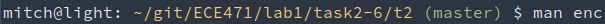
\includegraphics[scale=0.48]{t2p0.png}
    \end{center}{}
    \caption{using man on enc}
    \label{fig:t2p0}
\end{figure}

\begin{figure}[H]
    \begin{center}
        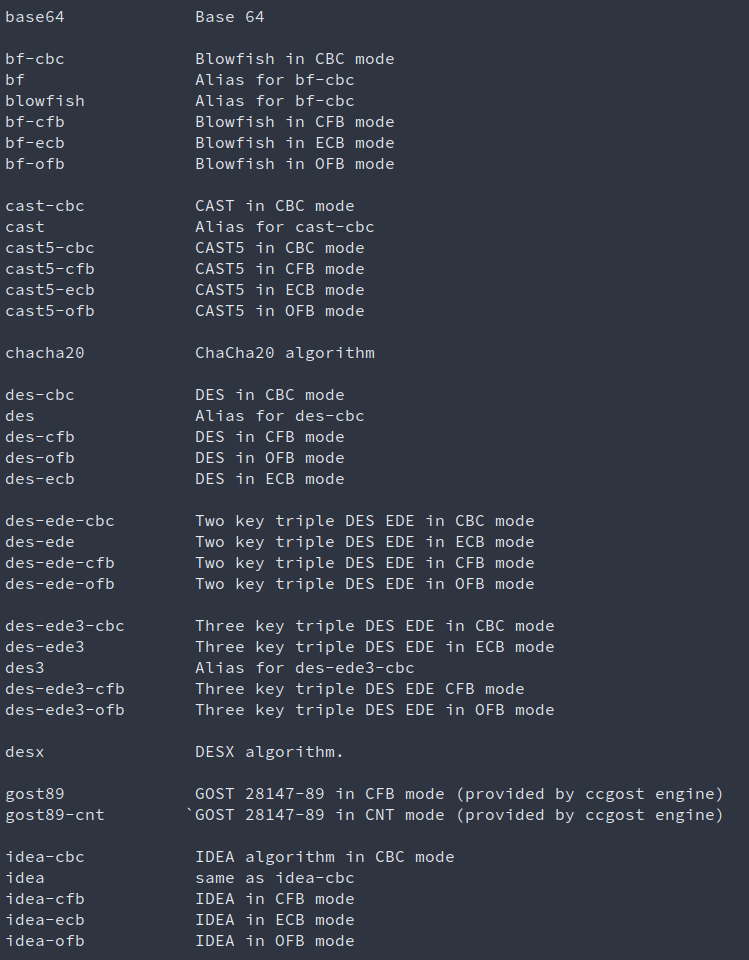
\includegraphics[scale=0.48]{t2p1.png}
    \end{center}{}
    \caption{encryption schemes from enc using man part 1}
    \label{fig:t2p1}
\end{figure}

\begin{figure}[H]
    \begin{center}
        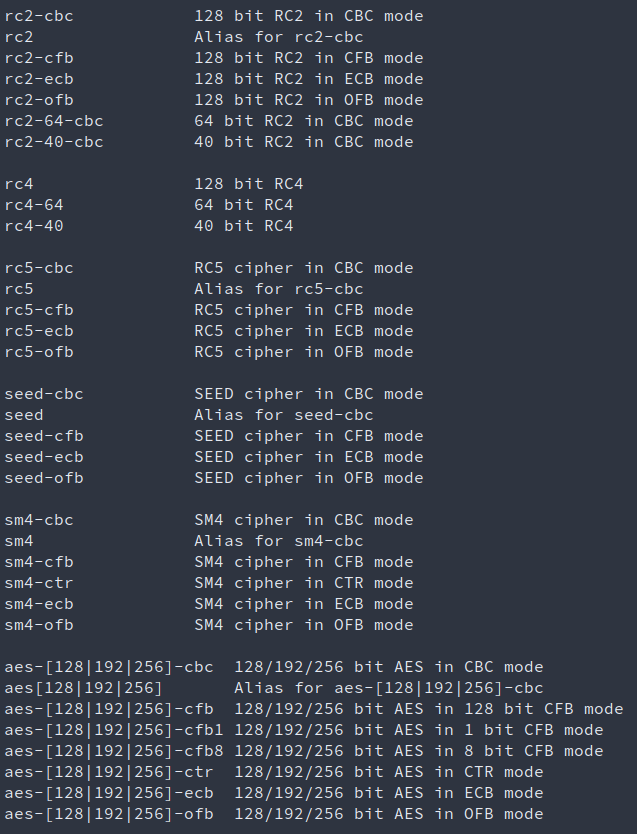
\includegraphics[scale=0.48]{t2p2.png}
    \end{center}{}
    \caption{encryption schemes from enc using man part 2}
    \label{fig:t2p2}
\end{figure}

\begin{figure}[H]
    \begin{center}
        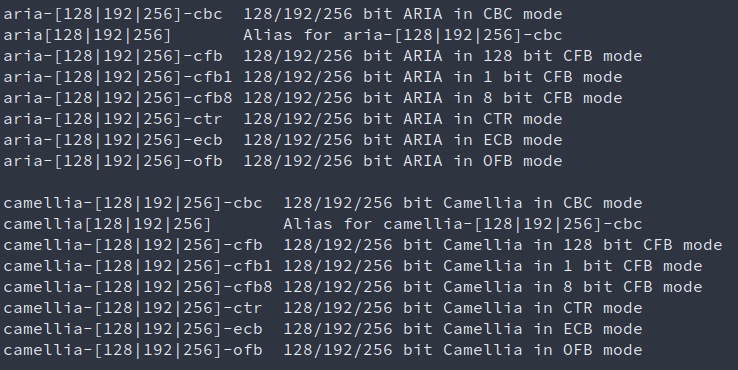
\includegraphics[scale=0.48]{t2p3.png}
    \end{center}{}
    \caption{encryption schemes from enc using man part 3}
    \label{fig:t2p3}
\end{figure}

Figure~\ref{fig:t2p1}, Figure~\ref{fig:t2p2} and Figure~\ref{fig:t2p3} show the results of the command shown in  Figure~\ref{fig:t2p0} which is an impresive amount of encryption schemes that could be used, most of which have 3 levels of bits that can be used to effectively make the algorithm more resistant to certain attacks such as brute force attacks.

This task requires us to try at least 3 different ciphers on the ciphertext. Just for fun, the following ciphers are used:

\begin{enumerate}
    \item bf-cbc
    \item aes-256-cbc
    \item aria-192-ecb
    \item camellia-256-ofb
\end{enumerate}


\end{document}
